\documentclass[conference]{IEEEtran}
\IEEEoverridecommandlockouts
% The preceding line is only needed to identify funding in the first footnote. If that is unneeded, please comment it out.
\usepackage{cite}
\usepackage{amsmath,amssymb,amsfonts}
\usepackage{epsfig,subfigure,multirow}
\usepackage{algorithmic}
\usepackage{graphicx}
\usepackage{textcomp}
\usepackage{xcolor, color}
\usepackage{romannum}
\usepackage[pagebackref=false]{hyperref}
\usepackage{array}
\usepackage{pstricks}
\usepackage{enumitem}
\usepackage{verbatim}
\usepackage{stfloats}
\usepackage[bookmarks=false]{}
\usepackage{aecompl}
\usepackage{mathrsfs}
\usepackage{arydshln}
\usepackage{mathtools} 
\usepackage{amsthm}
\usepackage{caption}
\usepackage{lipsum}
\usepackage{bm}
\usepackage{graphicx}
\usepackage{algorithm}
\usepackage{algorithmic}
\usepackage{comment}
\usepackage{booktabs}
\usepackage{tikz}
% \usepackage[a4paper, left=1.57 cm,
%             right=1.57 cm,
%             top=0.75in,
%             bottom=1in,]{geometry}

%\usepackage[cache=false]{minted}
\def \BibTeX{{\rm B\kern-.05em{\sc i\kern-.025em b}\kern-.08em
		T\kern-.1667em\lower.7ex\hbox{E}\kern-.125emX}}


\newtheorem{theorem}{Theorem}
\newtheorem{corollary}{Corollary}
\newtheorem{definition}{Definition}
\newtheorem{lemma}{Lemma}
\newtheorem{conjecture}{Conjecture}
\newtheorem{remark}{Remark}
\newtheorem{observation}{Observation}

\begin{document}
	
    \title{Optimal Communication-Computation Trade-off in Hierarchical Gradient Coding}
	
    \author{
	\IEEEauthorblockN{
		Ali Gholami\IEEEauthorrefmark{1}, Tayyebeh Jahani-Nezhad\IEEEauthorrefmark{1}, Kai Wan\IEEEauthorrefmark{2},  Giuseppe~Caire\IEEEauthorrefmark{1}
	}
	\IEEEauthorblockA{\IEEEauthorrefmark{1}Technische Universit\"at Berlin, 10587 Berlin, Germany, \{a.gholami, caire, t.jahani.nezhad\}@tu-berlin.de}%
	\IEEEauthorblockA{\IEEEauthorrefmark{2}Huazhong University of Science and Technology, China, kai\_wan@hust.edu.cn}%
	%\IEEEauthorblockA{\IEEEauthorrefmark{3}University of North Texas, Denton, TX 76203, USA, hua.sun@unt.edu}%
	%\IEEEauthorblockA{\IEEEauthorrefmark{4}University of Utah, Salt Lake City, UT 84112, USA, mingyue.ji@utah.edu}%
    }
	
    \maketitle
	
    \begin{abstract}
        In this paper, we study gradient coding in a hierarchical setting, where there are intermediate nodes between the server and the workers. This structure reduces the bandwidth requirements at the server, which is a  bottleneck in conventional gradient coding systems.  In this paper, the intermediate nodes, referred to as \textit{relays}, process the data received from workers and send the results to the server for the final gradient computation. Our main contribution is deriving the optimal communication-computation trade-off by designing a linear coding scheme inspired by coded computing techniques, considering straggling and adversarial nodes among both relays and workers. The processing of the data in the relays makes it possible to achieve both the relay-to-server and the worker-to-relay communication loads simultaneously optimal with regard to the computation load. 
    \end{abstract}

	
    \section{Introduction}
Distributed machine learning has emerged as an essential solution for the challenging task of training complex models with large datasets \cite{dean2012large,ahmed2013distributed,li2014communication,verbraeken2020survey}. In this approach, either the dataset or the model parameters are distributed across multiple servers that collaborate to train or evaluate the model. A commonly used scenario, particularly for deep neural networks, involves storing the model parameters on a server node while dividing the dataset among worker nodes. Each worker node then computes partial gradients of the model using its local dataset and sends the results to the server node, where they are aggregated to compute the gradient over the entire dataset. However, distributed machine learning faces several challenges. Some of the major ones include communication overhead, which arises from transferring large amounts of data such as gradient vectors \cite{li2014communication}; the computational cost per node; the issue of stragglers, or slow-performing nodes \cite{dean2013tail}; and adversarial nodes that may attempt to compromise the accuracy of the final results \cite{blanchard2017machine,chen2017distributed}. 

To address some of these challenges, \cite{tandon2017gradient} proposed a coded computing framework called \emph{gradient coding}, which enables the server node to efficiently collect and aggregate gradient vectors with minimal communication overhead while mitigating the impact of stragglers. In \cite{ye2018communication}, a trade-off between communication cost, computation load, and straggler tolerance was characterized in a homogeneous distributed system. \cite{jahani2021optimal} characterized the optimum communication cost for heterogeneous distributed systems with arbitrary data placement across worker nodes in the presence of stragglers and adversarial nodes. The paper also introduced a universal polynomial function and proposed an achievable scheme based on it. In \cite{wan2021distributed, wan2021tradeoff}, the gradient coding problem was generalized to scenarios where there is a user node which requests workers to compute a linearly separable function of the datasets, which is multiple linear combinations of the partial gradients. 
% In \cite{bitar2020stochastic,raviv2018gradient,charles2017approximate,glasgow2021approximate}, follow-up works on \textit{approximate} gradient coding have been proposed.
% Building on the insight that stochastic gradient descent (SGD) can function effectively with an unbiased approximation of the aggregated gradient vector, several follow-up works on gradient coding have been developed \cite{bitar2020stochastic,raviv2018gradient,charles2017approximate,glasgow2021approximate}.

Most studies on gradient coding have focused on the conventional server-worker star topology, where the server is connected to each worker through an individual link.  However, this architecture for distributed learning requires extensive resources, particularly at the server node, where high network bandwidth usage can create critical bottlenecks, especially in practical applications. 
% To overcome this challenge, some works have considered a hierarchical structure, where they consider intermediate nodes between the server and the workers. 
% %These intermediate nodes are directly connected to the workers, and they are responsible for doing some processing on the calculations done by the workers, that would otherwise be done on the server. 
% In \cite{prakash2020hierarchical, krishnan2023hierarchical}, the authors have considered the hierarchical gradient aggregation problem where workers are connected to helper nodes, and the helper nodes to the master. In this setting, being gradient aggregation, each worker has its individual local dataset and there is no overlap between the datasets of any group of workers.
To address this challenge,   hierarchical structures were considered that includes intermediate nodes between the server and the workers. In \cite{prakash2020hierarchical, krishnan2023hierarchical}, the authors consider the hierarchical gradient aggregation problem, where workers are connected to helper nodes, and the helper nodes are connected to the server. It was also assumed that each worker has its individual local dataset, with no overlap between the datasets of any group of workers.
In \cite{reisizadeh2019tree, bhattacharya2021improved, reisizadeh2021codedreduce, shah2024tree}, the authors studied the tree structure in gradient coding, where for each intermediate node there is a set of children nodes and a parent node. Each intermediate node has the responsibility of aggregating the partial gradients received from the children nodes and its own individual partial gradient and sends the result to the parent node. However, tree gradient coding schemes suffer from the high communication load, as they focus only on minimizing the computation cost of each worker node.
%\textcolor{red}{(anything related to the communication or computation? "The main drawback of hierarchical gradient schemes proposed in [17-22] is ......  ")}


In this paper, we propose an alternative scheme for hierarchical gradient coding, where  a server is connected to a group of \textit{relay} nodes, with each relay node connected to a group of \textit{workers}. The workers compute the partial gradients for the datasets assigned to them and send   linearly encoded vectors to their respective relays. The relay nodes can proceed computation on the data received from the workers and send the results  to the server. The proposed scheme enables the server to recover the sum of partial gradients from the messages received from the relays while coping with stragglers and adversarial nodes both among the relays and the workers. Our main contribution  lies in characterizing and achieving the optimal communication-computation trade-off through the design of a linear coding scheme based on polynomial functions, inspired by \cite{jahani2021optimal}. Besides, the proposed scheme enables heterogeneous data assignment across workers; this means the workers are allowed to have different computational power. The proposed hierarchical scheme significantly reduces the bandwidth requirement needed by the server compared to non-hierarchical gradient coding scenarios.
% We show that by this structure, we decrease the bandwidth requirement needed by the server, which exists in non-hierarchical gradient coding scenarios. 
A recent study on hierarchical gradient coding was proposed in~\cite{tang2024design}, which focuses solely on minimizing the computation load, whereas our approach extends the analysis to address the full communication-computation trade-off. 
% {\red SO OUR RESULT CAN COVER THEIR RESULTS??? HOWEVER, IN THEIR MODEL EACH RELAY CAN BE CONNECTED TO DIFFERENT NUMBERS OF USERS.}

% In a recent publication on arXiv \cite{tang2024design}, the authors consider a similar hierarchical setting in which the master is connected to edge nodes, and to each edge node a group of workers are connected. However, they only design a scheme for the case of minimum computation load, whereas we have extended the results to the entire trade-off of communication and computation. 

%The difference between this setting and the tree structure is that here the edge nodes do not have computation power and only possibly process the information received by the workers. They consider straggling workers in each cluster, along with straggling edge nodes. This structure is the same as ours in this paper.


%Unlike \cite{tang2024design} where the authors only consider the straggler-computation trade-off, in this paper we consider the more general case of communication-computation trade-off, which includes the aforementioned result. Using the polynomial coding approach in \cite{jahani2021optimal}, we have designed an achievable hierarchical gradient coding scheme, which we prove to be optimal considering the communication-computation curve. 


%\textcolor{red}{It is better to first introduce our paper and what we have done, then as a related work mention this recent work and compare it with ours. Using someone's paper we should not describe our structure.}
%In a recent published paper on arXiv \cite{tang2024design}, the authors consider a hierarchical setting in which the master is connected to edge nodes, and to each edge node a group of workers are connected. The difference between this setting and the tree structure is that here the edge nodes do not have computation power and only possibly process the information received by the workers. They consider straggling workers in each cluster, along with straggling edge nodes. This structure is the same as ours in this paper.









 
    %\noindent{\bf Notation:}
     %   Sets are denoted by calligraphic letters, vectors by boldface letters, and scalars with sans-serif symbols. 


    \section{Problem setting} \label{sec:problemsetting}
        
    In a typical supervised machine learning setting, given a training dataset $\mathcal{D}=\{(\mathbf{x}_i,y_i)\}_{i=1}^M$ for some integer $M$, where $\mathbf{x}_i \in \mathbb{R}^\ell$, $\ell\in\mathbb{N}$ is the $i$th input sample and $y_i \in \mathbb{R}$ the corresponding label, the goal is to learn the parameters $\mathbf{\Omega}$ (e.g., of neural network) by minimizing an empirical loss function $L(\mathcal{D};\mathbf{\Omega})=\frac
    {1}{|\mathcal{D}|}\sum_{i=1}^{M} L(\mathbf{x}_i,y_i;\mathbf{\Omega})$, where the optimization is solved by the gradient descent algorithm. The algorithm starts with an initial guess of $\mathbf{\Omega}$ denoted as $\mathbf{\Omega}^{(0)}$, which then in each iteration $t+1$ gets updated as
    % \begin{align}
        $\mathbf{\Omega}^{(t+1)}=f(\mathbf{\Omega}^{(t)}, \mathbf{g}^{(t)})$,
    % \end{align}
    where $\mathbf{g}^{(t)}\in\mathbb{R}^d$ is the gradient of the loss function defined as $\mathbf{g}^{(t)}:=\nabla L(\mathcal{D};\mathbf{\Omega}^{(t)})=\frac{1}{|\mathcal{D}|}\sum_{i=1}^M \nabla L(\mathbf{x}_i,y_i;\mathbf{\Omega}^{(t)})$, where $\nabla$ indicates the gradient w.r.t $\mathbf{\Omega}^{(t)}$.

    Consider a setting with a server and multiple worker nodes. %including up to $s\in\mathbb{N}$ stragglers and up to $a\in\mathbb{N}$ adversarial worker nodes %\textcolor{red}{I added $s$ and $a$ here. I would be better to mention stragglers and adversaries at this point. Can we define the relationship between $a_1,a_2$ and $s_1,s_2$ with $a$ and $s$ accordingly?} 
    %\textcolor{blue}{For the adversarial nodes, we should clarify the following: by "adversary," we refer to nodes that may send incorrect computations but do not exhibit any other malicious behavior}.
    The training dataset $\mathcal{D}$ is partitioned into $K\in\mathbb{N}$ equal-sized datasets,  $\mathcal{D}=\{\mathcal{D}_1, ...,\mathcal{D}_K\}$.
    In this setting, there are $N_1$ clusters, where cluster $i$ contains $N_2^{(i)}$ workers. The workers in each cluster are connected to a relay and the relays are connected to the server. The datasets are assigned to the workers in the data placement phase. Then each worker computes the gradients of the assigned datasets using the current value of $\mathbf{\Omega}$. The partial gradient of dataset $\mathcal{D}_k$ with the learning parameters $\mathbf{\Omega}^{(t)}$ at iteration $t$, is denoted by $\mathbf{g}_k^{(t)} \in \mathbb{R}^d$, which we simplify to $\mathbf{g}_k$ since we only consider the gradient descent algorithm only for one iteration. The ultimate goal of the server is to compute $\mathbf{g}=\sum_{k=1}^K \mathbf{g}_k$. 

    Worker $j$ in cluster $i$ (or worker $(i,j)$) is denoted by $W_{i,j}$, and the set of datasets assigned to it is denoted by $\Gamma_{i,j}$, where apparently $\Gamma_{i,j} \neq \emptyset$. Additionally, we denote the set of datasets assigned to relay-$i$ by $\Gamma_i$. When a dataset is assigned to relay-$i$, it implies that it has been assigned to at least one worker in cluster $i$. Each worker $(i,j)$ encodes the locally computed partial gradients of datasets in $\Gamma_{i,j}$ using a linear encoding function 
    % \begin{align}
       $ \mathcal{E}_{(i,j)}: (\mathbb{R}^d)^{|\Gamma_{i,j}|} \rightarrow \mathbb{R}^{C_2^{(i)}},$
    % \end{align}
    where $C_2^{(i)}$ denotes the size of the vector sent by each worker in cluster $i$ to its relay. The encoded vector computed by worker $(i,j)$ is denoted by $\Tilde{\mathbf{g}}_{(i,j)} \in \mathbb{R}^{C_2^{(i)}}$;
    \begin{align}
        \Tilde{\mathbf{g}}_{(i,j)} = \mathcal{E}_{(i,j)}(\{\mathbf{g}_k\}_{k: \mathcal{D}_k \in \Gamma_{(i,j)}}).
    \end{align}

    Relay-$i$ receives the encoded vectors sent by the workers in its cluster, considering $s_2^{(i)} \in \mathbb{N}$ \textit{stragglers} and $a_2^{(i)} \in \mathbb{N}$ \textit{adversarial} workers in cluster-$i$. The straggling nodes are those with failed links or very delayed communication, and by ``adversary”, we refer to nodes that may send incorrect computations but do not exhibit any other malicious behavior. Then using the encoded vectors received from non-straggling workers, denoted by the set $\mathcal{F}_i$,  relay-$i$ encodes a new message $\Tilde{\mathbf{g}}_{i} \in \mathbb{R}^{C_1}$ by using a linear encoding as
    \begin{align}
        \Tilde{\mathbf{g}}_{i} = \mathcal{E}_i(\mathcal{F}_i, \{\Tilde{\mathbf{g}}_{(i,j)}\}_{(i,j)\in \mathcal{F}_i}),
    \end{align}
    where 
    % \begin{align}
      $  \mathcal{E}_i: \mathcal{F}_i \times (\mathbb{R}^{C_2^{(i)}})^{|\mathcal{F}_i|} \rightarrow \mathbb{R}^{C_1}. $
    % \end{align}

    Relay-$i$ sends the encoded vector $\Tilde{\mathbf{g}}_{i}$ to the server. The server tolerates $s_1\in\mathbb{N}$ straggling and $a_1\in\mathbb{N}$ adversarial relays. After receiving the encoded vectors from non-straggling relays, denoted by the set $\mathcal{F}$, the server recovers the desired gradient vector as
    \begin{align}
        \mathbf{g} = \mathcal{H}(\mathcal{F}, \{\Tilde{\mathbf{g}}_{i}\}_{i \in \mathcal{F}}),
    \end{align}
    where 
    % \begin{align}
       $ \mathcal{H}: \mathcal{F} \times (\mathbb{R}^{C_1})^{|\mathcal{F}|} \rightarrow \mathbb{R}^d$. 
    % \end{align}

    Note that the communication cost from workers to the relays is defined by $C_2^{(i)}$ in cluster $i$ and from relays to the server by $C_1$. A communication tuple $(C_1,C_2^{(1)}, ..., C_2^{(N_1)})$ is achievable if there exists a hierarchical gradient coding scheme with encoding functions $(\{\mathcal{E}_{(i,j)}\}_{i\in [N_1], j\in [N_2^{(i)}]}, \{\mathcal{E}_{(i)}\}_{i\in [N_1]})$ and decoding function $\mathcal{H}$, such that the server can correctly recover the desired gradient vector $\mathbf{g}$. The minimum values of $C_1$ and $C_2^{(i)}$s among all achievable schemes are denoted by $C_1^*$ and $C_2^{(i)*}$ respectively. 

    \subsection{Data Assignment}
    %The datasets can be arbitrarily distributed, which is referred to as heterogeneous data assignment \textcolor{red}{Our setting is not heterogeneous data assignment}. 
    % In this paper we impose an additional condition on the data assignment as follows.
    %Let $\mathcal{A}_k^{(w)}$ denote the set of workers to which the dataset $\mathcal{D}_k$ is assigned, with its size denoted as
    % The size of this set is denoted by $r_T^k$;
    %$r_T^k=|\mathcal{A}_k^{(w)}|$. %We assume that the size of this set is the same for all $k \in [K]$, denoted by $r_T$;
    %\begin{align}
     %   r_T \triangleq |\mathcal{A}_1^{(w)}|=...=|\mathcal{A}_K^{(w)}|
    %\end{align}
    Let $\mathcal{A}_k$ denote the set of clusters to which the dataset $\mathcal{D}_k$ is assigned. Dataset $\mathcal{D}_k$ is considered assigned to a cluster if it is assigned to at least one worker within that cluster. The size of this set is denoted as  $r_1^k=|\mathcal{A}_k|$. Naturally we should have that $r_1^k \leq N_1$. %Similarly, we assume that the size of this set is the same for all  $k\in [K]$, denoted by $r_1$;
    %\begin{align}
     %   r_1 \triangleq |\mathcal{A}_1^{(c)}|=...=|\mathcal{A}_K^{(c)}|.
    %\end{align}
    If dataset $\mathcal{D}_k$ is assigned to cluster $i$, then the set of workers in that cluster having the dataset is denoted by $\mathcal{A}_k^{(i)}$, and its size is denoted by $r_{2,i}^k=|\mathcal{A}_k^{(i)}|$, and this value can not be greater than $N_2^{(i)}$; $r_{2,i}^k \leq N_2^{(i)}$.
    

    
    \section{Main Results}
    \begin{theorem}
        For the hierarchical gradient coding problem defined in Section \ref{sec:problemsetting}, the minimum communication loads are charaterized by
        \begin{align}
            C^*_1 = \frac{d}{m_1}, C^{(i)*}_2 = \frac{d}{m_1m^{(i)}_2},
        \end{align}
        where $m_1=r_1-2a_1-s_1$ and $m^{(i)}_2=r_{2,i}-2a^{(i)}_2-s^{(i)}_2$, in which
        \begin{align}
            r_1 &= \min_{k\in [K]} r_1^k, \\
            r_{2,i} &= \min_{\substack{k\in [K] \\ k:\mathcal{D}_{k}\in\Gamma_{i}}} r_{2,i}^k.
        \end{align}
    \end{theorem}

     
    \begin{proof}
        The proof of achievability is presented in Section \ref{sec:generalscheme}, where we describe the general scheme in detail.
        
       For the converse, we first model the system as consisting of one server and multiple clusters, where each cluster contains a relay with its children workers. In fact, each cluster can be viewed as a giant worker node. This transforms the problem into a conventional gradient coding setting with a server connected to multiple workers. From the result in \cite[Theorem 1]{jahani2021optimal}, it follows that $C^*_1 = \frac{d}{m_1}$.

        Additionally, for any linear encoding and general decoding functions, we prove for cluster $i$ that $C^{(i)}_2 \ge \frac{d}{m_1m^{(i)}_2}$. To do so, we show that the task in each cluster is equivalent to a conventional gradient coding setting.
        Since the size of the vector sent by relay-$i$ to the server is $C_1$, and relay-$i$ does a linear encoding on the received vectors from the workers inside the cluster, $\Tilde{\mathbf{g}}_{i}$ could be written as 
        \begin{align}
            \Tilde{\mathbf{g}}_{i} = \mathbf{A}_{C_1 \times |\Gamma_i|d} 
            \begin{bmatrix}
               \vdots \\
               \mathbf{g}_k \\
               \vdots \\
            \end{bmatrix}_{k\in \Gamma_i}.
        \end{align}
        Now if we divide each partial gradient into $m_1$ equally-sized parts as $\mathbf{g}_k=
            \begin{bmatrix}
               \mathbf{g}_k^1 \\
               \vdots \\
               \mathbf{g}_k^{m_1} \\
            \end{bmatrix}$
        (or the zero-padded version of each partial gradient if $m_1 \nmid d$), then 
        \begin{align}
            \Tilde{\mathbf{g}}_{i} = \mathbf{A}_{C_1 \times m_1|\Gamma_i|\frac{d}{m_1}} 
            \begin{bmatrix}
               \vdots \\
               \mathbf{g}_k^1 \\
               \vdots \\
               \mathbf{g}_k^{m_1} \\
               \vdots \\
            \end{bmatrix}_{k\in \Gamma_i}.
        \end{align}

        If we consider $C_1=C_1^*=\frac{d}{m_1}$, then this corresponds to a conventional gradient coding scenario with $m_1|\Gamma_i|$ datasets each of size $\frac{d}{m_1}$. Remember that this does not change the value of $r_{2,i}$. In such a scenario, the server would want to compute the total gradient which is of the form
        \begin{align}
             \mathbf{g} = \mathbf{A}'_{\frac{d}{m_1} \times m_1|\Gamma_i|\frac{d}{m_1}} 
             \begin{bmatrix}
               \vdots \\
               \mathbf{g}_k^1 \\
               \vdots \\
               \mathbf{g}_k^{m_1} \\
               \vdots \\
            \end{bmatrix},
        \end{align}
        where
        \begin{align}
            \mathbf{A}'_{\frac{d}{m_1} \times m_1|\Gamma_i|\frac{d}{m_1}}=
            \begin{bmatrix}
               1,0,...,0, & 1,0,...,0, & ... & 1,0,...,0 \\
               0,1,...,0, & 0,1,...,0, & ... & 0,1,...,0 \\
               \vdots & \vdots & ... & \vdots \\
               0,0,...,1, & 0,0,...,1, & ... & 0,0,...,1
            \end{bmatrix}.
        \end{align}
        Since both $\mathbf{A}$ and $\mathbf{A}'$ are full-rank matrices with the same size, we can say that the correspondence exists. Since the straggling and adversarial worker nodes in cluster $i$ is $s_2^{(i)}$ and $a_2^{(i)}$ respectively, using the conventional gradient coding, we would have
        \begin{align}
            C_2^{(i)}=\frac{d/m_1}{m_2^{(i)}}=\frac{d}{m_1m_2^{(i)}},
        \end{align}
        where $m_2^{(i)}=r_{2,i}-2a_2^{(i)}-s_2^{(i)}$. For any $C_1 > \frac{d}{m_1}$, the problem in each cluster corresponds to more than a single conventional gradient coding (the problem can be divided to at least one standard gradient coding). So $C_2^*$ occurs when $C_1^*$ occurs. This completes the proof. 
    \end{proof}
    % \vspace{-4mm}
    \begin{remark}
        %In a symmetrical setting where the parameters of each cluster, including the number of workers and stragglers, are the same, 
        The result presented in \cite{tang2024design} is a special case of our proposed scheme, specifically when  $r_1=s_e+1$ and $r_{2,i}=s_w+1$ for each cluster-$i$, without considering adversarial nodes. Here $s_e$ and $s_w$
  represent the number of stragglers among relays and in each cluster, respectively, as defined
  in \cite{tang2024design}. Note that, in this case, both the relay to server and the worker to relay communication loads will be  $C_1=C_{2}^{(i)}=d, \forall i \in [N_1]$, matching the result in \cite{tang2024design}.
        %The setting in \cite{tang2024design} is similar to the setting in this paper. However, they only consider the minimum computation load for each worker, which is equivalent to the case of $r_1=s_1+1$ and $r_2=s_2+1$ (not considering adversarial nodes). Their communication loads is $C_1=C_2=d$, which can also be derived by our optimal scheme. \textcolor{red}{I revised it as follows, if it is true, replace it with the existing remark:
        %The result presented in \cite{tang2024design} is a special case of our proposed scheme, specifically when  $r_1=s_1+1$ and $r_2=s_2+1$ without considering adversarial nodes.}
    \end{remark}

    %\begin{remark}
     %   The coding framework proposed in this paper has the flexibility to be easily extended to the case where the parameters of each cluster is different; namely the number of workers, stragglers, and adversarial workers. This is possible because the encoding and decoding in each cluster is done based on a local polynomial tailored to the cluster. 
    %\end{remark}

    \begin{remark}
    % The optimal communication loads are achieved simultaneously using the polynomial coding technique.
In the proposed scheme, the optimal communication loads are achieved simultaneously through the use of polynomial coding techniques in both the workers and the relays. In fact, the relays do not only forward the received vectors; instead, they serve as intermediate nodes that perform computations on the information received from the workers.
    % This has been made possible through the decoding and encoding of linearly encoded vectors in the relays. 
    % In fact, in the proposed scheme the relays do not just simply forward the received vectors, they are intermediate nodes to process the information received from the workers. 
    \end{remark}

    \begin{remark}
        Let us compare the hierarchical setting to a non-hierarchical setting with the same parameters. For simplicity of comparison, we assume the parameters of each cluster in the hierarchical setting is the same; all having $s_2$ stragglers and $N_2$ workers. This would lead to a total of $N_1s_2$ straggling workers. Using the result in \cite{jahani2021optimal}, the total communication load received by the server from all workers in the non-hierarchical scheme with the same parameters would be $\frac{N_1N_2d}{r_T-N_1s_2}$, where $r_T$ denotes the minimum number of copies of each dataset among workers. However, in the proposed hierarchical scheme, the load received by the server (considering no straggling and no adversarial relays) would be $\frac{N_1d}{r_1}$. Since $r_T$ would be at most $r_1N_2$,  it follows that the total load in the hierarchical setting is less than that in the non-hierarchical setting, highlighting the advantage of the hierarchical structure with respect to bandwidth limitations. %\textcolor{red}{Is this remark correct? Why does the communication depend on $N_1N_2$ rather than $d$? }
    \end{remark}
    %\textcolor{red}{I am not sure about placing these remarks here, but it’s up to you.
    % \vspace{-5mm}
    \section{Proposed Scheme Through an Example}
   In this section, we explain the proposed scheme through a motivating example. For simplicity, here we consider a homogeneous data assignment among workers, where each worker possesses the same number of datasets. Figure \ref{fig:diagram exmp} illustrates a hierarchical setting consisting of $N_1=3$ clusters, each containing $3$ workers, i.e. $N_2^{(1)}=N_2^{(2)}=N_2^{(3)}=3$. The dataset is partitioned into $K=9$ equal-sized datasets, and the data assignment is performed such that  $r_1=2$, and  $r_{2,1}=r_{2,2}=r_{2,3}=2$. 
    \begin{figure}[ht]
    \centering
    \resizebox{0.9\columnwidth}{!}{%
    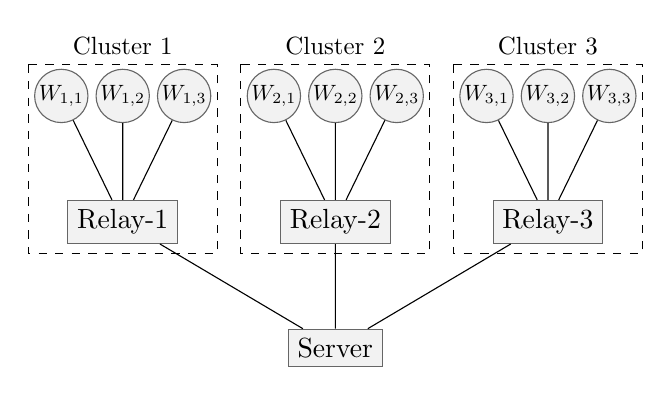
\begin{tikzpicture} [xscale=0.6, yscale=0.8,
    roundnode/.style={circle, draw=black!60, fill=black!5},
    squarednode/.style={rectangle, draw=black!60, fill=black!5},
    ]
        \node[roundnode,inner sep=0.5pt] (1) at (0.2,0) {\scalebox{0.8}{$W_{1,1}$}};
        \node[roundnode,inner sep=0.5pt] (2) at (1.5,0) {\scalebox{0.8}{$W_{1,2}$}};
        \node[roundnode,inner sep=0.5pt] (3) at (2.8,0) {\scalebox{0.8}{$W_{1,3}$}};
        \node[roundnode,inner sep=0.5pt] (4) at (4.7,0) {\scalebox{0.8}{$W_{2,1}$}};
        \node[roundnode,inner sep=0.5pt] (5) at (6,0) {\scalebox{0.8}{$W_{2,2}$}};
        \node[roundnode,inner sep=0.5pt] (6) at (7.3,0) {\scalebox{0.8}{$W_{2,3}$}};
        \node[roundnode,inner sep=0.5pt] (7) at (9.2,0) {\scalebox{0.8}{$W_{3,1}$}};
        \node[roundnode,inner sep=0.5pt] (8) at (10.5,0) {\scalebox{0.8}{$W_{3,2}$}};
        \node[roundnode,inner sep=0.5pt] (9) at (11.8,0) {\scalebox{0.8}{$W_{3,3}$}};

        \node[squarednode] (10) at (1.5,-2) {Relay-1};
        \node[squarednode] (11) at (6,-2) {Relay-2};
        \node[squarednode] (12) at (10.5,-2) {Relay-3};

        \draw[dashed] (-0.5, 0.5) rectangle (3.5,-2.5);
        \draw[dashed] (4, 0.5) rectangle (8,-2.5);
        \draw[dashed] (8.5, 0.5) rectangle (12.5,-2.5);
        
        \draw[-] (1) -- (10);
        \draw[-] (2) -- (10);
        \draw[-] (3) -- (10);

        \draw[-] (4) -- (11);
        \draw[-] (5) -- (11);
        \draw[-] (6) -- (11);

        \draw[-] (7) -- (12);
        \draw[-] (8) -- (12);
        \draw[-] (9) -- (12);

        \node[squarednode] (13) at (6,-4) {Server};
        
        \draw[-] (10) -- (13);
        \draw[-] (11) -- (13);
        \draw[-] (12) -- (13);
        \node at (1.5, .8) {\scalebox{0.9}{Cluster 1}};
        \node at (6, 0.8) {\scalebox{0.9}{Cluster 2}};
        \node at (10.5, 0.8) {\scalebox{0.9}{Cluster 3}};
        
    \end{tikzpicture}
    }
    \caption{Hierarchical setting used in the motivating example.}
    \label{fig:diagram exmp}
    % \vspace{-8mm}
    \end{figure}
    Consider the dataset assignment is performed as follows.
    \begin{align*} 
        \Gamma_{1,1} &= \{\mathcal{D}_1, \mathcal{D}_3, \mathcal{D}_7, \mathcal{D}_9\},
        \Gamma_{1,2} = \{\mathcal{D}_1, \mathcal{D}_3, \mathcal{D}_4, \mathcal{D}_6\}, \\
        \Gamma_{1,3} &= \{\mathcal{D}_4, \mathcal{D}_6, \mathcal{D}_7, \mathcal{D}_9\}, \\
        \Gamma_{2,1} &= \{\mathcal{D}_1, \mathcal{D}_2, \mathcal{D}_7, \mathcal{D}_8\},
        \Gamma_{2,2} = \{\mathcal{D}_1, \mathcal{D}_2, \mathcal{D}_4, \mathcal{D}_5\}, \\
        \Gamma_{2,3} &= \{\mathcal{D}_4, \mathcal{D}_5, \mathcal{D}_7, \mathcal{D}_8\}, \\
        \Gamma_{3,1} &= \{\mathcal{D}_2, \mathcal{D}_3, \mathcal{D}_8, \mathcal{D}_9\},
        \Gamma_{3,2} = \{\mathcal{D}_2, \mathcal{D}_3, \mathcal{D}_5, \mathcal{D}_6\}, \\
        \Gamma_{3,3} &= \{\mathcal{D}_5, \mathcal{D}_6, \mathcal{D}_8, \mathcal{D}_9\},
    \end{align*}
    which leads that
    \begin{align*}
     &   \Gamma_{1} = \{\mathcal{D}_1, \mathcal{D}_3, \mathcal{D}_4, \mathcal{D}_6, \mathcal{D}_7, \mathcal{D}_9\}, \\
       & \Gamma_{2} = \{\mathcal{D}_1, \mathcal{D}_2, \mathcal{D}_4, \mathcal{D}_5, \mathcal{D}_7, \mathcal{D}_8\}, \\
       & \Gamma_{3} = \{\mathcal{D}_2, \mathcal{D}_3, \mathcal{D}_5, \mathcal{D}_6, \mathcal{D}_8, \mathcal{D}_9\}.
    \end{align*}
    We assume that none of the relays are stragglers or adversaries; however, within each cluster, there is a single straggler, i.e., $a_1=s_1=0, a_2^{(1)}=a_2^{(2)}=a_2^{(3)}=0, s_2^{(1)}=s_2^{(2)}=s_2^{(3)}=1$. We then define $m_1$ and $m_2^{(i)}$ as $m_1 \triangleq r_1-2a_1-s_1=2, m_2^{(1)}\triangleq r_{2,1}-2a_2^{(1)}-s_2^{(1)}=1, m_2^{(2)}\triangleq r_{2,2}-2a_2^{(2)}-s_2^{(2)}=1, m_2^{(3)}\triangleq r_{2,3}-2a_2^{(3)}-s_2^{(3)}=1$. Let us assume that each partial gradient is divided into $m_1=2$ equal-sized parts, represented as $\mathbf{g}_k = (\mathbf{g}_k[1], \mathbf{g}_k[2])$. 
    %Subsequently, since $m_2^{(1)}=m_2^{(2)}=m_2^{(3)}=1$, each of these parts is further divided into $1$ equal-sized parts, represented as $\mathbf{g}_k[i] = (\mathbf{g}_k[i,1])$. It is evident that $\mathbf{g}_k[i]=\mathbf{g}_k[i,1]$. 
    Let us focus on cluster-1. For this cluster, since $m_2^{(1)}=1$, each of these parts is further divided into $m_2^{(1)}=1$ equal-sized parts, represented as $\mathbf{g}_k[i] = (\mathbf{g}_k[i,1])$. It is evident that $\mathbf{g}_k[i]=\mathbf{g}_k[i,1]$. Each worker in this cluster sends a linear combination of the elements of its computed partial gradients to relay-1 as follows
    \begin{align*}
        \Tilde{\mathbf{g}}_{(1,1)} &\triangleq \frac{8}{9} \mathbf{g}_{1}[1] + \frac{2}{3} \mathbf{g}_{3}[1]  + \frac{2}{3} \mathbf{g}_{7}[1] + \frac{1}{2} \mathbf{g}_{9}[1] \nonumber \\
        &-\frac{1}{3} \mathbf{g}_{1}[2] - \frac{2}{9} \mathbf{g}_{3}[2] - \frac{1}{4} \mathbf{g}_{7}[2] - \frac{1}{6} \mathbf{g}_{9}[2], \\
        \Tilde{\mathbf{g}}_{(1,2)} &\triangleq \frac{4}{9} \mathbf{g}_{1}[1] + \frac{1}{3} \mathbf{g}_{3}[1]  - \frac{4}{3} \mathbf{g}_{4}[1] - \mathbf{g}_{6}[1] \nonumber \\
        &-\frac{1}{6} \mathbf{g}_{1}[2] - \frac{1}{9} \mathbf{g}_{3}[2] + \frac{1}{2} \mathbf{g}_{4}[2] + \frac{1}{3} \mathbf{g}_{6}[2], \\
        \Tilde{\mathbf{g}}_{(1,3)} &\triangleq -\frac{8}{3} \mathbf{g}_{4}[1] - 2 \mathbf{g}_{6}[1]  - \frac{2}{3} \mathbf{g}_{7}[1] - \frac{1}{2} \mathbf{g}_{9}[1] \nonumber \\
        &+\mathbf{g}_{4}[2] + \frac{2}{3} \mathbf{g}_{6}[2] + \frac{1}{4} \mathbf{g}_{7}[2] + \frac{1}{6} \mathbf{g}_{9}[2].
    \end{align*}
    Note that each worker in the cluster only sends a vector of size $\frac{d}{2}$ to the relay.
    Now consider the following polynomial function, referred to as Intra-Cluster  encoding polynomial for cluster-1: 
    \begin{align*}
        \mathbf{f}_{\text{intraC}}^{(1)}(x_2)&=
         \mathbf{g}_{1}[1] \frac{4(x_2-3)}{-9} + \mathbf{g}_{3}[1] \frac{x_2-3}{-3} + \mathbf{g}_{4}[1] \frac{4(x_2-1)}{-3} \\
        &+ \mathbf{g}_{6}[1] \frac{x_2-1}{-1} + \mathbf{g}_{7}[1] \frac{2(x_2-2)}{-3} + \mathbf{g}_{9}[1] \frac{x_2-2}{-2} \nonumber \\
        &+ \mathbf{g}_{1}[2] \frac{x_2-3}{6} + \mathbf{g}_{3}[2] \frac{x_2-3}{9} + \mathbf{g}_{4}[2] \frac{x_2-1}{2} \\
        &+ \mathbf{g}_{6}[2] \frac{x_2-1}{3} + \mathbf{g}_{7}[2] \frac{x_2-2}{4} + \mathbf{g}_{9}[2] \frac{x_2-2}{6}.
    \end{align*}
One can verify that $\Tilde{\mathbf{g}}_{(1,i)}$ sent by worker $W_{(1,i)}$ is equal to
   $\mathbf{f}_{\text{intraC}}^{(1)}(x_2=i)$. Since this polynomial is of degree 1, it can be recovered by any two evaluations. Although there is a straggler among the workers in cluster-1, relay-1 will still be able to recover $\mathbf{f}_{\text{intraC}}^{(1)}(x_2)$ . Then, relay-1 computes $\tilde{\mathbf{g}}_1\triangleq\mathbf{f}_{\text{intraC}}^{(1)}(x_2=0)$ and sends the result, which is a vector of size $\frac{d}{2}$, to the server. 
    For cluster-$2$ and cluster-$3$, the corresponding Intra-Cluster polynomials are defined as follows.
    \begin{align*}
        \mathbf{f}_{\text{intraC}}^{(2)}(x_2)&=
        \mathbf{g}_{1}[1] \frac{x_2-3}{-3} + \mathbf{g}_{2}[1] \frac{x_2-3}{1} + \mathbf{g}_{4}[1] \frac{x_2-1}{-1} \nonumber\\
        &+ \mathbf{g}_{5}[1] \frac{3(x_2-1)}{1} + \mathbf{g}_{7}[1] \frac{x_2-2}{-2} + \mathbf{g}_{8}[1] \frac{3(x_2-2)}{2} \nonumber \\
        &+ \mathbf{g}_{1}[2] \frac{x_2-3}{6} + \mathbf{g}_{2}[2] \frac{x_2-3}{-3} + \mathbf{g}_{4}[2] \frac{x_2-1}{2} \nonumber\\
        &+ \mathbf{g}_{5}[2] \frac{x_2-1}{-1} + \mathbf{g}_{7}[2] \frac{x_2-2}{4} + \mathbf{g}_{8}[2] \frac{x_2-2}{-2}, \\
    % \end{align*}
    % \begin{align*}
        \mathbf{f}_{\text{intraC}}^{(3)}(x_2)&\hspace{-1mm}=\hspace{-1mm}
        \mathbf{g}_{2}[1] \frac{8(x_2-3)}{3} + \mathbf{g}_{3}[1] \frac{2(x_2-3)}{3} + \mathbf{g}_{5}[1] \frac{8(x_2-1)}{1} \nonumber\\
        &+ \mathbf{g}_{6}[1] \frac{2(x_2-1)}{1} + \mathbf{g}_{8}[1] \frac{4(x_2-2)}{1} + \mathbf{g}_{9}[1] \frac{x_2-2}{1} \nonumber \\
        &+ \mathbf{g}_{2}[2] \frac{x_2-3}{-1} + \mathbf{g}_{3}[2] \frac{x_2-3}{-3} + \mathbf{g}_{5}[2] \frac{3(x_2-1)}{1} \nonumber\\
        &+ \mathbf{g}_{6}[2] \frac{x_2-1}{-1} + \mathbf{g}_{8}[2] \frac{3(x_2-2)}{-2} + \mathbf{g}_{9}[2] \frac{x_2-2}{-2}.
    \end{align*}
    Similarly, worker $(i,j)$, for $i=2,3$ and $j=1,2,3$, sends the value of $\mathbf{f}_{\text{intraC}}^{(i)}(x_2=j)$ to its parent relay. Relay-$i$ tolerating one straggler, is then able to interpolate $\mathbf{f}_{\text{intraC}}^{(i)}(x_2)$.
    Next, relay-$i$ computes $ \Tilde{\mathbf{g}}_{i} \triangleq\mathbf{f}_{\text{intraC}}^{(i)}(x_2=0)$ and  sends the result to the server, which is as follows. 
    \begin{align*}
        \Tilde{\mathbf{g}}_{1}&= 
        % &\triangleq\mathbf{f}_{\text{intraC}}^{(1)}(x_2=0)= \\
        \frac{4}{3} \mathbf{g}_{1}[1]+\mathbf{g}_{3}[1]+\frac{4}{3} \mathbf{g}_{4}[1]+\mathbf{g}_{6}[1]+\frac{4}{3} \mathbf{g}_{7}[1]+\mathbf{g}_{9}[1] \nonumber \\
        & -\frac{1}{2} \mathbf{g}_{1}[2]-\frac{1}{3} \mathbf{g}_{3}[2]-\frac{1}{2} \mathbf{g}_{4}[2]-\frac{1}{3} \mathbf{g}_{6}[2]-\frac{1}{2} \mathbf{g}_{7}[2]-\frac{1}{3} \mathbf{g}_{9}[2], \\
        % \end{align*}
        % \begin{align*}
              \Tilde{\mathbf{g}}_{2} &=
              % &\triangleq\mathbf{f}_{\text{intraC}}^{(2)}(x_2=0)= \\
        \mathbf{g}_{1}[1]-3\mathbf{g}_{2}[1]+\mathbf{g}_{4}[1]-3\mathbf{g}_{5}[1]+\mathbf{g}_{7}[1]-3\mathbf{g}_{8}[1] \nonumber \\
        & -\frac{1}{2} \mathbf{g}_{1}[2]+\mathbf{g}_{2}[2]-\frac{1}{2}\mathbf{g}_{4}[2]+\mathbf{g}_{5}[2]-\frac{1}{2}\mathbf{g}_{7}[2]+\mathbf{g}_{8}[2], \\
      %   \end{align*}
      % \begin{align*}
                \Tilde{\mathbf{g}}_{3}& =
                % &\triangleq\mathbf{f}_{\text{intraC}}^{(3)}(x_2=0)= \\
         -8\mathbf{g}_{2}[1]-2\mathbf{g}_{3}[1]-8\mathbf{g}_{5}[1]-2\mathbf{g}_{6}[1]-8\mathbf{g}_{8}[1]-2\mathbf{g}_{9}[1] \nonumber \\
        & +3\mathbf{g}_{2}[2]+\mathbf{g}_{3}[2]+3\mathbf{g}_{5}[2]+\mathbf{g}_{6}[2]+3\mathbf{g}_{8}[2]+\mathbf{g}_{9}[2]. 
      \end{align*}
  
    Now consider the following polynomial, referred to as Cluster-to-Server encoding polynomial.
    \begin{align*}
        &\mathbf{f}_{\text{C2S}}(x_1)= 
         \left( \mathbf{g}_{1}[1] \frac{x_1-3}{-3} + \mathbf{g}_{2}[1] \frac{x_1-1}{-1} + \mathbf{g}_{3}[1] \frac{x_1-2}{-2} \right. \nonumber \\ 
        &+ \left. \mathbf{g}_{4}[1] \frac{x_1-3}{-3} + \mathbf{g}_{5}[1] \frac{x_1-1}{-1} + \mathbf{g}_{6}[1] \frac{x_1-2}{-2} \right. \nonumber \\ 
        &+ \left. \mathbf{g}_{7}[1] \frac{x_1-3}{-3} + \mathbf{g}_{8}[1] \frac{x_1-1}{-1} + \mathbf{g}_{9}[1] \frac{x_1-2}{-2} \right) (x_1+1) \nonumber \\
        &+ \left( \mathbf{g}_{1}[2] \frac{x_1-3}{-4} + \mathbf{g}_{2}[2] \frac{x_1-1}{-2} + \mathbf{g}_{3}[2] \frac{x_1-2}{-3} + \mathbf{g}_{4}[2] \frac{x_1-3}{-4} \right. \nonumber \\ 
        &+ \left. \mathbf{g}_{5}[2] \frac{x_1-1}{-2} + \mathbf{g}_{6}[2] \frac{x_1-2}{-3} + \mathbf{g}_{7}[2] \frac{x_1-3}{-4} + \mathbf{g}_{8}[2] \frac{x_1-1}{-2} \right. \nonumber \\
        &+ \left. \mathbf{g}_{9}[1] \frac{x_1-2}{-3} \right) (-x_1).
    \end{align*}
    This polynomial has two main properties: (1) $\Tilde{\mathbf{g}}_{i}$, sent by relay-$i$, is equal to an evaluation of $\mathbf{f}_{\text{C2S}}(x_1)$ at the point $x_1=i$. This polynomial is of degree 2 and can be recovered by any three evaluations. Since in this example, there are no stragglers among the relays, the server can recover this polynomial upon receiving     
    $\Tilde{\mathbf{g}}_{1}$, $\Tilde{\mathbf{g}}_{2}$, and $\Tilde{\mathbf{g}}_{3}$. (2) One can verify that $\mathbf{f}_{\text{C2S}}(x_1=0)$ is equal to $\mathbf{g}[1]=\sum_{k=1}^{9}\mathbf{g}_k[1]$, and  $\mathbf{f}_{\text{C2S}}(x_1=-1)$ is equal to $\mathbf{g}[2]=\sum_{k=1}^{9}\mathbf{g}_k[2]$, thereby recovering $\mathbf{g}=(\mathbf{g}[1], \mathbf{g}[2])$. 

Note that since each worker and relay sends a linear combination of the $\mathbf{g}_k[i]$s, each of size  $\frac{d}{2}$, the communication costs are $C_1=C_2=\frac{d}{2}$. 

    \section{The General  Hierarchical Gradient Coding Scheme} \label{sec:generalscheme}
 In this section, we formally describe the proposed gradient coding scheme in a hierarchical setting, which achieves optimal communication load under a heterogeneous data assignment among workers; the number of datasets assigned to each worker is not necessarily the same and can be different based on the computational power of each worker. Building on the universal polynomial function proposed in \cite{jahani2021optimal}, we extend this idea to design two encoding polynomials, referred to as the \emph{Intra-Cluster} and \emph{Cluster-to-Server} encoding polynomials. These polynomials are specifically tailored to the hierarchical setting, enabling efficient communication and computation in this structure.
    % The general proposed scheme is based on designing polynomials referred to as \textit{universal polynomials} to determine the task of each worker and relay. The scheme is based on linear coding on the elements of the partial gradients.
    
Each partial gradient, which is a vector of size $d$, is partitioned into $m_1$ parts as $\mathbf{g}_k=(\mathbf{g}_k[1], \dots, \mathbf{g}_k[m_1])$, used to design the cluster-to-server polynomial. Furthermore, to design the intra-cluster polynomial in cluster $c$, each part is further divided into $m_2^{(c)}$ subparts, represented as $\mathbf{g}_k[i]=(\mathbf{g}_k[i,1], \dots, \mathbf{g}_k[i,m_2^{(c)}])$. Consequently, each partial gradient can be expressed by $\mathbf{g}_k=(\mathbf{g}_k[1,1], ..., \mathbf{g}_k[m_1,m_2^{(c)}])$, where $m_1 \triangleq r_1-2a_1-s_1$ and $m_2^{(c)} \triangleq r_{2,c}-2a_2^{(c)}-s_2^{(c)}$. If $m_1m_2^{(c)} \nmid d$, we can zero pad the partial gradient.
   
    % We first define variables $m_1$ and $m_2$ as $m_1 \triangleq r_1-2a_1-s_1$ and $m_2 \triangleq r_2-2a_2-s_2$. We partition each partial gradient into $m_1m_2$ elements; $\mathbf{g}_k=(\mathbf{g}_k[1,1], ..., \mathbf{g}_k[m_1,m_2])$.

    % The coding is designed in two layers; the \textit{outer code} and the \textit{inner code}. The outer code refers to what relays should compute, and the inner code refers to what workers should compute, which relies on the outer code. We therefore begin with the design of the outer code in the following.
    \subsection{Design of the Encoding Polynomials}
The encoding process is designed in two layers: the Intra-Cluster part and the Cluster-to-Server part. The first layer specifies the computations to be carried out by the relays, while the second layer defines the computations to be performed by the workers. These two polynomials are interconnected and are designed based on the system parameters and the data assignment.
We begin by describing the design of the Cluster-to-Server encoding polynomial below.\\    
\noindent\textbf{Design of the Cluster-to-Server Encoding: }  Let $\alpha_1^{(1)}, ..., \alpha_{N_1}^{(1)}$ and $\beta_1^{(1)}, ..., \beta_{m_1}^{(1)}$ be $N_1+m_1$ distinct values  chosen from $\mathbb{R}$. We aim to find a polynomial function, denoted by $\mathbf{f}_{\text{C2S}}(x_1)$, which has the following properties:
 % We want to define a polynomial $f_{outer}(x_1)$, referred to as \textit{the outer code polynomial} with the following properties.
    \begin{enumerate}[leftmargin=*, noitemsep]
        \item  $\mathbf{f}_{\text{C2S}}(\alpha_i^{(1)})$ is a function of the datasets in $\Gamma_i$.  Here, $\alpha_i^{(1)}$ represents the point where $\mathbf{f}_{\text{C2S}}(x_1)$ is evaluated by relay-$i$. Since relay-$i$ has access only to the datasets in $\Gamma_i$,  its computations are limited to those datasets. During the scheme, the computed evaluation by relay-$i$ is sent to the server.
        \item  $\mathbf{f}_{\text{C2S}}(x_1)$ is a polynomial of degree $N_1-2a_1-s_1-1$. This ensures that the server can recover the polynomial using $N_1-2a_1-s_1$ evaluations, even in the presence of $s_1$ straggler relays whose evaluations are not received and $a_1$ adversarial relays that may provide incorrect evaluations.
        \item At point $\beta_i^{(1)}$, $\mathbf{f}_{\text{C2S}}(x_1)$ satisfies the following condition:
        \begin{align*}
           \mathbf{f}_{\text{C2S}}(\beta_i^{(1)}) = \sum_{k=1}^K \mathbf{g}_k[i] = \mathbf{g}[i].
        \end{align*}
      When the server recovers $\mathbf{f}_{\text{C2S}}(x_1)$, it computes the  $i$-th  element of the desired gradient by evaluating the polynomial at $\beta_i^{(1)}$, thereby recovering the entire gradient vector.
    \end{enumerate}
 % \textbf{1) $f_{outer}(\alpha_i^{(1)})$ should be a function of datasets in $\Gamma_i$. } In fact, $\alpha_i^{(1)}$ is the point on which $f_{outer}(x_1)$ will be evaluated by relay $i$. Naturally, relay $i$ is only able to do computation on datasets in $\Gamma_i$.
 
    % \textbf{2) } This is because we want the polynomial to be recoverable by the evaluations of the relays. Since $s_1$ of the relays are stragglers and their evaluations are not received by the server, and to combat the $a_1$ adversary relays which do not necessarily send the accurate evaluations, it is necessary that the server be able to recover the polynomial with $N_1-2a_1-s_1$ evaluations. 

    % \textbf{3) $\mathbf{f}_{\text{C2S}}(\beta_j^{(1)}) = \sum_{k=1}^K \mathbf{g}_k[j] = \mathbf{g}[j]$. } When the server recovers $\mathbf{f}_{\text{C2S}}(x_1)$, it calculates the element $i$ of the desired gradient by evaluating the polynomial in $\beta_i^{(1)}$; therefore recovering the whole gradient.

  In order to design $\mathbf{f}_{\text{C2S}}(x_1)$,  we first define the polynomial $\mathbf{p}_{l_1}(x_1)$ as follows.
    \begin{align}
        \mathbf{p}_{l_1}(x_1)=\sum_{k=1}^{K} \mathbf{g}_{k}[l_1] \prod^{N_1}_{\substack{i=1 \\ i:\mathcal{D}_{k}\notin\Gamma_{i}}} \frac{x_1-\alpha^{(1)}_{i}}{\beta^{(1)}_{l_1}-\alpha^{(1)}_{i}},
    \end{align}
    %where $\mathbf{g}_{k}[l_1] = (\mathbf{g}_{k}[l_1,1], ..., \mathbf{g}_{k}[l_1,m_2])$. 
    The property of this polynomial is that $\mathbf{p}_{l_1}(\beta_{l_1}^{(1)})=\sum_{k=1}^K \mathbf{g}_k[l_1]$, and  $\mathbf{p}_{l_1}(\alpha_{n}^{(1)})$ depends only on the partial gradients of datasets in $\Gamma_n$.
   The polynomial $\mathbf{f}_{\text{C2S}}(x_1)$ with the mentioned properties is created as follows.
    \begin{align} \label{eq:outer}
        \mathbf{f}_{\text{C2S}}(x_1)=\sum_{l_1=1}^{m_1} \bigg(\mathbf{p}_{l_1}(x_1)  \prod^{m_1}_{\substack{u_1=1 \\ u_1 \neq l_1}} \frac{x_{1}-\beta^{(1)}_{u_1}}{\beta^{(1)}_{l_1}-\beta^{(1)}_{u_1}}\bigg).
    \end{align}
    % \textcolor{red}{here $\mathbf{f}_{\text{C2S}}(\beta_{l_1}^{(1)})=\sum_{l_1=1}^{m_1}\sum_{k=1}^{K}\mathbf{g}_k[l_1]$, am I right? It is not equal to the third condition. No, if you put $\beta_i^{(1)}$, because of the multiplication on the right, only the term $l_1=i$ remains in the sum.}
    
    In the proposed scheme, relay-$n$ sends the evaluation of  $\mathbf{f}_{\text{C2S}}(x_1)$ at point $x_1=\alpha_n^{(1)}$ to the server. More precisely, 
    % The task of each relay $n$ would be $\Tilde{\mathbf{g}}_n = \mathbf{f}_{\text{C2S}}(\alpha_n^{(1)})$;
    \begin{align*} 
        \Tilde{\mathbf{g}}_n\triangleq
        \sum_{l_1=1}^{m_1} \left(\sum_{k=1}^{K} \mathbf{g}_{k}[l_1] \prod^{N_1}_{\substack{i=1 \\ i:\mathcal{D}_{k}\notin\Gamma_{i}}} \frac{\alpha_n^{(1)}-\alpha^{(1)}_{i}}{\beta^{(1)}_{l_1}-\alpha^{(1)}_{i}} \right)  \prod^{m_1}_{\substack{u_1=1 \\ u_1 \neq l_1}} \frac{\alpha_n^{(1)}-\beta^{(1)}_{u_1}}{\beta^{(1)}_{l_1}-\beta^{(1)}_{u_1}},
    \end{align*}
    is sent to the server by relay-$n$ where $\mathbf{g}_{k}[l_1] = (\mathbf{g}_{k}[l_1,1],...,\mathbf{g}_{k}[l_1,m_2^{(n)}])$, thereby $\Tilde{\mathbf{g}}_n = (\Tilde{\mathbf{g}}_n[1],...,\Tilde{\mathbf{g}}_n[m_2^{(n)}])$. Since this is a linear combination of $\mathbf{g}_{k}[l_1]$s of size $\frac{d}{m_1}$, the relay-to-server communication cost would be $C_1=\frac{d}{m_1}$. Note that $\Tilde{\mathbf{g}}_n$ is a linear combination of the partitions of the partial gradients of datasets in $\Gamma_n$.

 \noindent   \textbf{Design of the Intra-Cluster Encoding: } For each cluster $n$, we need a separate Intra-Cluster encoding polynomial accustomed to the corresponding Cluster-to-Server encoding and $\Tilde{\mathbf{g}}_n$. Let $\alpha_1^{(2)}, ..., \alpha_{N_2^{(n)}}^{(2)}$ and $\beta_1^{(2)}, ..., \beta_{m_2^{(n)}}^{(2)}$ be $N_2^{(n)}+m_2^{(n)}$ distinct values chosen from $\mathbb{R}$. We aim to find a polynomial function, denoted by  $\mathbf{f}_{\text{intraC}}^{(n)}(x_2)$, which has the following properties:
\begin{enumerate}[leftmargin=*, noitemsep]
    \item  $\mathbf{f}_{\text{intraC}}^{(n)}(\alpha_j^{(2)})$ is a function of datasets in $\Gamma_{(n,j)}$.  Specifically, $\alpha_j^{(2)}$ represents the point at which $\mathbf{f}_{\text{intraC}}^{(n)}(x_2)$ is evaluated by worker $(n,j)$ and then sent to relay-$n$. Worker-$(n,j)$ can only perform computations on the datasets within $\Gamma_{(n,j)}$. 
    \item  $\mathbf{f}_{\text{intraC}}^{(n)}(x_2)$ is a polynomial of degree $N_2^{(n)}-2a_2^{(n)}-s_2^{(n)}-1$.  This degree is chosen to ensure that the polynomial can be recovered from the evaluations of the workers in the cluster. Since $s_2^{(n)}$ workers are stragglers whose evaluations are not received by the relay, and $a_2^{(n)}$ workers may behave adversarially by sending incorrect evaluations, it is necessary for the relay to recover the polynomial using  $N_2^{(n)}-2a_2^{(n)}-s_2^{(n)}$ evaluations. 
    \item  At point $\beta_j^{(2)}$, $\mathbf{f}_{\text{intraC}}^{(n)}(x_2)$ satisfies the following condition:
    \begin{align*}
     \mathbf{f}_{\text{intraC}}^{(n)}(\beta_j^{(2)}) = \tilde{\mathbf{g}}_n[j].   
    \end{align*}
   In other words, after relay-$n$ recovers
 $\mathbf{f}_{\text{intraC}}^{(n)}(x_2)$, it calculates the $j$-th element of $\tilde{\mathbf{g}}_n$  by evaluating the polynomial at $\beta_j^{(2)}$, thereby computing the entire vector $\tilde{\mathbf{g}}_n$.
\end{enumerate}
    % \textbf{1) $\mathbf{f}_{\text{intraC}}^{(n)}(\alpha_j^{(2)})$ should be a function of datasets in $\Gamma_{(n,j)}$. } In fact, $\alpha_j^{(2)}$ is the point on which $\mathbf{f}_{\text{intraC}}^{(n)}(x_2)$ will be evaluated by worker $(n,j)$. Naturally, worker $(n,j)$ is only able to do computation on datasets in $\Gamma_{(n,j)}$. 

    % \textbf{2) $\mathbf{f}_{\text{intraC}}^{(n)}(x_2)$ should be a polynomial of degree $N_2-2a_2-s_2-1$. } This is because we want the polynomial to be recoverable by the evaluations of the workers in the cluster. Since $s_2$ of the workers are stragglers and their evaluations are not received by the relay, and to combat the $a_2$ adversary workers which do not necessarily send the accurate evaluations, it is necessary that the relay be able to recover the polynomial with $N_2-2a_2-s_2$ evaluations. 

    % \textbf{3) $\mathbf{f}_{\text{intraC}}^{(n)}(\beta_j^{(2)}) = \Tilde{\mathbf{g}}_n[j]$. } When the relay recovers $\mathbf{f}_{\text{intraC}}^{(n)}(x_2)$, it calculates the element $j$ of the outer code by evaluating the polynomial in $\beta_j^{(2)}$; therefore recovering the whole outer code $\Tilde{\mathbf{g}}_n$.

    We first define the polynomial $\mathbf{p}_{l_2}^{(n)}(x_2)$ as follows.
    \begin{align*}
        &\mathbf{p}_{l_2}^{(n)}(x_2)= \\ &\sum_{l_1=1}^{m_1}\hspace{-1mm}\left(\sum_{k=1}^{K} \mathbf{g}_{k}[l_1,l_2]\prod^{N_1}_{\substack{i=1 \\ i:\mathcal{D}_{k}\notin\Gamma_{i}}} \frac{\alpha_n^{(1)}-\alpha^{(1)}_{i}}{\beta^{(1)}_{l_1}-\alpha^{(1)}_{i}}
        \prod^{N_2^{(n)}}_{\substack{j=1 \\ j:\mathcal{D}_{k}\notin\Gamma_{n,j}}} \hspace{-2mm}\frac{x_2-\alpha^{(2)}_{j}}{\beta^{(2)}_{l_2}-\alpha^{(2)}_{j}} \right) \nonumber\\ &\prod^{m_1}_{\substack{u_1=1 \\ u_1 \neq l_1}} \frac{\alpha_1^{(1)}-\beta^{(1)}_{u_1}}{\beta^{(1)}_{l_1}-\beta^{(1)}_{u_1}}.
    \end{align*}
    The property of this polynomial is that $\mathbf{p}_{l_2}^{(n)}(\beta_{l_2}^{(2)})= \Tilde{\mathbf{g}}_n[l_2]$, and $\mathbf{p}_{l_2}^{(n)}(\alpha_{j}^{(2)})$ depends only on the partial gradients of datasets in $\Gamma_{(n,j)}$. The Intra-Cluster encoding polynomial for cluster-$n$, denoted by $ \mathbf{f}_{\text{intraC}}^{(n)}(x_2)$, is defined as follows. 
    \begin{align}
        \mathbf{f}_{\text{intraC}}^{(n)}(x_2) =
        \sum_{l_2=1}^{m_2^{(n)}} \mathbf{p}_{l_2}^{(n)}(x_2) \prod^{m_2^{(n)}}_{\substack{u_2=1 \\ u_2 \neq l_2}} \frac{x_{2}-\beta^{(2)}_{u_2}}{\beta^{(2)}_{l_2}-\beta^{(2)}_{u_2}}.
    \end{align}
    In the proposed scheme, the task of worker-$(n,j)$ is to calculate 
    $\mathbf{f}_{\text{intraC}}^{(n)}(\alpha_j^{(2)})$, i.e.,
    \begin{align} \label{eq:workertask}
        \Tilde{\mathbf{g}}_{n,j} \triangleq \sum_{l_2=1}^{m_2^{(n)}} \mathbf{p}_{l_2}^{(n)}(\alpha_j^{(2)}) \prod^{m_2^{(n)}}_{\substack{u_2=1 \\ u_2 \neq l_2}} \frac{\alpha_j^{(2)}-\beta^{(2)}_{u_2}}{\beta^{(2)}_{l_2}-\beta^{(2)}_{u_2}},
    \end{align}
and send the result to relay-$n$. Since this is a linear combination of $\mathbf{g}_{k}[l_1,l_2]$s of size $\frac{d}{m_1m_2^{(n)}}$, the worker-to-relay communication cost would be $C_2=\frac{d}{m_1m_2^{(n)}}$.
\subsection{The Proposed Hierarchical Gradient Coding Scheme}
   With the provided description, the proposed scheme proceeds as follows:
\begin{enumerate}
    \item \textbf{ Worker-to-Relay Transmission.} The worker $(n,j)$ computes  $\Tilde{\mathbf{g}}_{n,j}$ as defined in \eqref{eq:workertask}, and sends the result to relay-$n$. 
    \item \textbf{ Calculating Intra-Cluster Polynomial by the Relay.} Upon receiving $\Tilde{\mathbf{g}}_{n,j}$ from non-straggling workers, relay-$n$ recovers $\mathbf{f}_{\text{intraC}}^{(n)}(x_2)$, which is of degree $N_2^{(n)}-2a_2^{(n)}-s_2^{(n)}-1$. 
    \item \textbf{ Relay-to-Server Transmission.} Relay-$n$,  utilizing the third property of the Intra-Cluster polynomial, computes $\Tilde{\mathbf{g}}_{n} = (\Tilde{\mathbf{g}}_{n}[1],...,\Tilde{\mathbf{g}}_{n}[m_2^{(n)}])$ and sends it to the server.
    \item  \textbf{ Calculating Cluster-to-Server Polynomial by the Server.} The server, having received $\Tilde{\mathbf{g}}_{n}$ from non-straggling relays, recovers $\mathbf{f}_{\text{C2S}}(x_1)$,  which is of degree  $N_1-2a_1-s_1-1$. 
    \item \textbf{Final Gradient Recovery.}  Using the third property of the Cluster-to-Server polynomial, the server calculates the aggregated partial gradients ${\mathbf{g}} = ({\mathbf{g}}[1],...,{\mathbf{g}}[m_1])$.
    
\end{enumerate}
%     \noindent \textbf{1) Worker-to-Relay Transmission.} The worker $(n,j)$ computes  $\Tilde{\mathbf{g}}_{n,j}$ as defined in \eqref{eq:workertask}, and sends the result to relay-$n$. 
    
%    \noindent \textbf{2) Calculating Intra-Cluster Polynomial by the Relay.} Upon receiving $\Tilde{\mathbf{g}}_{n,j}$ from non-straggling workers, relay-$n$ recovers $\mathbf{f}_{\text{intraC}}^{(n)}(x_2)$, which is of degree $N_2-2a_2-s_2-1$. 


%    \noindent \textbf{3) Relay-to-Server Transmission.} Relay-$n$,  utilizing the third property of the Intra-Cluster polynomial, computes $\Tilde{\mathbf{g}}_{n} = (\Tilde{\mathbf{g}}_{n}[1],...,\Tilde{\mathbf{g}}_{n}[m_2])$ and sends it to the server.

%  \noindent   \textbf{4) Calculating Cluster-to-Server Polynomial by the Server.} The server, having received $\Tilde{\mathbf{g}}_{n}$ from non-straggling relays, recovers $\mathbf{f}_{\text{C2S}}(x_1)$,  which is of degree  $N_1-2a_1-s_1-1$. 

% \noindent\textbf{5) Final Gradient Recovery.}  Using the third property of the Cluster-to-Server polynomial, the server calculates the aggregated partial gradients ${\mathbf{g}} = ({\mathbf{g}}[1],...,{\mathbf{g}}[m_1])$.
    
    
    % \paragraph*{Acknowledgement}
    % The work of A.~Gholami, T.~Jahani-Nezhad, and G.~Caire was partially funded by the ERC Advanced Grant N. 789190, CARENET. The work of K.~Wan was partially funded by NSFC-12141107. The work of H.~Sun was supported in part by NSF under Grant CCF-2007108, Grant CCF-2045656, and Grant CCF-2312228. The work of M.~Ji was partially funded by NSF Award 2312227 and CAREER Award 2145835. 
     
\bibliographystyle{IEEEtran}
 \bibliography{references}
 	
 %\appendices
 	 
 	


	
\end{document}


